\chapter{User Documentation} % User guide
\label{ch:user}

In this chapter, Mini Ericsson Orchestrator Cloud Manager is explained from an end-user perspective. Initially, a brief introduction to the cloud concepts is detailed. Then the tools used in front-end and back-end are introduced. Afterwards, an instruction to install and run the system is provided as well as all the requirements for the usage of this system. In conclusion, explanations on how to use each part of the application are given.

\section{Cloud}
\label{sec:cloud}
What is \emph{the cloud}?

Due to the boom in cloud computing in recent years, \emph{the cloud} as a term is fully integrated into the lives of ordinary people. The cloud refers to the servers that are accessed over the Internet, along with the software and databases that run on those servers~\cite{what-is-the-cloud}. By using the cloud, users and companies do not have to manage physical servers themselves or run software applications on their own machines. The cloud enables users to access the same applications and files from almost any device, because the computing and storage take place on servers in a remote data center, instead of the user device storage. For example, Gmail stores emails and attachments on google drive cloud storage allowing users to access their emails and files via any internet-connected device. Such benefits also include data security, unlimited storage capacity, backup, and data restoration.

If we look at the relationship between a user and the cloud, the examples detailed above cover the uses of the cloud. In short, it can be said that all usage is based on storing certain data.

However, if we will get a view from a different perspective, the developer's side, the field of the application will be tremendously widened. The focus shifts from storing data to processing data. In general, applications require increasing computing capacity. As a consequence of the growing demand for memory, the demand for processors has increased.

In fierce business competitions, there is a growing burden on developers. Diverting to cloud computing reduces IT and operating costs. For example, as the cloud vendor is used to update and maintain servers, they do not need to do it manually every time. This is really useful for small businesses when they are not able to afford internal infrastructure but can outsource their infrastructure needs affordably by means of the cloud. Moreover, international companies are operating easily by using the cloud, since employees and customers can access the same files and applications from any place.

Ericsson Orchestrator Cloud Manager allows cloud providers to build and grow cloud infrastructure for applications and services. It became necessary due to problems examining development opportunities. In connection with this, it is also worthwhile to review what is cloud computing.

\subsection{Cloud computing}
Humans use cloud computing without even realizing it. Using an online service to send an email, watch TV or movies, edit documents, or store pictures and other files, it is likely that it is cloud computing that makes it all possible in the background. So cloud computing is the delivery of computing services — including servers, storage, databases, networking, and software to offer faster innovation, and flexible resources. Customers usually pay for the cloud services they use, which helps to lower operating costs, run infrastructure more efficiently, and scale as their business needs change~\cite{cloud-computing}.

Benefits of cloud computing other than eliminating capital expenses are productivity, speed, and performance. Cloud companies have their own data centers where servers and/or data storage are located. Cloud data centers are regularly upgraded to the latest generation of fast and efficient computing hardware. The advantage is reduced network latency for applications and greater economies of scale over a single data center. Vast amounts of computing resources can be provisioned in minutes, which gives businesses a lot of flexibility and decreases pressure on capacity planning. When it comes to performance, it is about the time saved by not setting up hardware, software patching, and other time-consuming IT management tasks. Cloud computing takes away the need for many of these tasks, so developers can spend time on achieving more important business goals~\cite{what-is-cloud-computing}.

The initial cloud computing services are barely a decade old, nevertheless, small start-ups to international companies are embracing the technology for all kinds of reasons. By utilizing cloud computing services, users can create cloud-native applications, store, recover and analyze data as well as deliver software on demand.

\subsection{Docker Container}
A container is a standard unit of software package that includes the software code and all its dependencies, so the application runs quickly and reliably regardless of the computing environment~\cite{docker-container}.

Docker containers can be stored in image files and they are easy to build on their own executable software packages that contain everything you need to run an application: code, system tools, required system libraries, and settings.

Container image files become containers at runtime and in the case of Docker containers – images become containers when they run on the Docker Engine. The Docker Engine is available for Linux, MacOS, and Windows operating systems. In such containers, stored software is always the same and can run regardless of the infrastructure. The containers isolate the software from its environment and ensure that the software works uniformly. I am using the docker container to set up the PostgreSQL database. This is done by building an image from a Dockerfile. Dockerfile is a text file, it consists of all the commands needed to build a given image. 

\subsection{Kubernetes}
Container orchestration is the automation of much of the operational effort required to run containerized workloads and services. This includes a broad range of tasks software teams need to manage a container’s lifecycle, including deployment, provisioning, networking, scaling, load balancing, and so on.

If we are thinking about load-based handling of containers, Kubernetes can be considered one of the most common choices. It allows developers to easily build containerized applications and services, as well as scale, schedule, and monitor those containers. It is a great choice to have an already proven container for an orchestration solution need. Because of this, Kubernetes is currently the most popular container for orchestration platforms. While there are other options for container orchestration, such as Docker Swarm or Apache Mesos, Kubernetes has become the industry standard. Several of the world’s largest companies use it, and a significant portion of them is also involved in its development. Kubernetes contributes large-scale container capabilities, a dynamic contributor community, the growth of cloud-native application development, and the widespread availability of Kubernetes tools~\cite{kubernetes}. So, I used Kubernetes to provide me with the platform where the user is able to deploy and delete several resources such as \textit{ReplicaSet}, \textit{ControllerRevision}, and more. 

\subsubsection{Pods}
The smallest execution units are called Pods in a Kubernetes cluster. One or more containers are enclosed in a pod instead of one cluster running on cluster nodes. The common resources and local network are shared in a pod by applications which makes it easy to communicate between applications. Pods use a kubelet on each node to communicate with Kubernetes API and the rest of the cluster. Kubernetes can automatically recreate the pod to attain the desired scalability as the load increases.

\subsubsection{Nodes}
Node is the smallest unit of the compute hardware in a Kubernetes cluster. Nodes form a layer of abstraction like containers. One can think of a node as a basic resource with power and memory, then they can be identified with each other. All of them form the Kubernetes cluster. As needs alter, the Kubernetes cluster automates distributing of workloads. Nodes are immediately removed from the cluster when they are failed. In case of failure, new nodes replace them.

\subsubsection{Clusters}
A collection of nodes called Kubernetes cluster. They can be both physical servers or virtual machines. The User is always managing a cluster when utilizing Kubernetes. At least one instance of the Kubernetes control plane needs to run on a node, and at least one node for pods to execute on. On the condition that nodes are added or removed from the cluster, the cluster itself will automatically redistribute the load as necessary.

\subsection{Cloud Management Database}
Cloud Management Database stores the records for resources and services. It is a central repository that reflects the presence and state of objects in all infrastructure managers managed by Ericsson Orchestrator Cloud Manager. In other words, the Cloud Management Database stores all cloud objects and their attributes, including those that are instantiated in the VIM zones. PostgreSQL is used in the project as the cloud management database to be in charge of storage services.

\section{Install Guide}
\label{sec:install-guide}

\subsection{Back-End Tools}
Back-End development of the project was built up by Java Spring Boot with Spring Framework as the main programming language and PostgreSQL as a database tool. The followings explain each one of them in a brief description.

\subsubsection{Spring Framework}
Spring is the world's most popular Java framework for its speed, productivity, and simplicity. With the help of the Spring framework, Java programming becomes faster, easier, and safer for everyone.

``We use a lot of the tools that come with the Spring framework and reap the benefits of having a lot of the out of the box solutions, and not having to worry about writing a ton of additional code—so that really saves us some time and energy.'' Sean Graham,  Application Transformation Lead~\cite{why-spring}.

Spring has lots of trusted libraries that have been proven by developers in the whole world. Tech companies like Google, Microsoft, and many others have given their contributions to this framework. Spring brings solutions to everyday activities such as online shopping, streamings, or an immense amount of other innovations. The framework is able to create almost any application client can imagine by reason of third-party libraries and extensions. Spring is capable of building both secure cloud-based microservice for the web and complex flowing data streams for the companies.

\subsubsection{Java Spring Boot}
Java Spring Boot is a tool that develops web applications and microservices with Spring Framework quicker and more simple~\cite{java-spring-boot}. Spring Framework offers built-in assistance for common tasks that an application needs to perform. Here include data binding, type conversion, validation, exception handling, and more. Spring Boot is really useful when developers need to deploy microservices-based architectures into the cloud since Spring Cloud has supporting libraries and patterns. This transforms how you approach programming tasks, especially, Java related. Once you work on Spring Boot, you will notice fast start-up, shutdown, and optimized execution. Representational State Transfer (REST) APIs are developed by Spring Boot in Mini Ericsson Orchestrator Cloud Manager to establish communication between client and server over HTTP.

\subsubsection{PostgreSQL}
PostgreSQL is an advanced, enterprise-class open-source relational database that supports both SQL (relational) and JSON (non-relational) querying. It is a highly stable database, backed by more than 20 years of development which has contributed to its high levels of integrity, resilience, and correctness. PostgreSQL is used as a primary database for many web applications as well as mobile and analytics applications~\cite{postgresql}. It supports the most popular programming languages such as Python, Java, C/C+, JavaScript (Node.js), and Go.

The benefits of PostgreSQL are abundant features and extensions, reliability and standards compliance, and open source license. PostgreSQL owns robust feature sets including point-in-time recovery, tablespaces, nested transactions, a refined query planner/optimizer, and write ahead logging. It also supports international character sets, multi-byte character encodings, Unicode, and it is locale-aware for sorting, case-sensitivity, and formatting. PostgreSQL is a highly fault-tolerant database because of its write-ahead logging. It has full support for foreign keys, views, joins, and stored procedures, in many different languages. PostgreSQL source code is accessible under an open-source license, allowing you to use, modify, and implement it as you want at no charge~\cite{what-is-the-postgresql}. PostgreSQL provided me with storage where all the details about the users, created packages, and deployed resources into Kubernetes are kept.

\subsection{Front-End Tools}
Front-End development of the project has been prepared by React JS, React-Bootstrap, Material UI, HTML, and CSS are used. The followings explain each one of them in a brief description.

\subsubsection{React JS}
React what is also known as React.js or ReactJS is a free and open-source front-end JavaScript library for creating user interfaces based on UI components. It is sustained by Meta and a group of individual developers and companies. React can be used as a fundamental in the development of single-page, mobile, or even server-rendered applications with frameworks. Nevertheless, React is only troubled with state management and rendering that state to the DOM. Consequently, React applications usually requires the use of supplementary libraries for routing and other client-side functionalities~\cite{react-js-wiki}.

\subsubsection{React-Bootstrap}
React-Bootstrap replaces the Bootstrap JavaScript. Each one of the components has been created from scratch which converts into a true React component. In this case, dependencies like jQuery and others are unnecessary. React-Bootstrap has improved alongside React JS which is making it the perfect choice for UI design. It is well-suited to all types of Bootstrap themes, which gives a consistent appearance and maintains uniformity in the application~\cite{react-bootstrap}.

\subsubsection{Material UI}
Material UI is an open-source, front-end framework for React components. This framework is built using Leaner Style Sheets (LESS) which is a backward-compatible language extension for CSS. While developing front-end graphics of the application Material UI provides a high-quality digital experience based on Google's Material Design. Its main focuses are on providing bold and crisp designs, for example, it creates text fields by focusing on how components reflect the light and cast shadows~\cite{material-ui-react}.

\subsubsection{HTML}
HTML which stands for Hyper Text Markup Language is the standard markup language for creating Web pages. It describes the formation of a Web page and consists of a sequence of components. Each component of the HTML helps to label the content which makes it easy for the user to understand the interface~\cite{html-intro}.

\subsubsection{CSS}
Cascading Style Sheets (CSS) is a style sheet language used for describing the presentation of a document written in HTML or in other markup languages. CSS provides the layout, fonts, and color which improve content accessibility by providing more flexibility and control in the specification of presentation characteristics. It can control the layout of multiple web pages all at the same time~\cite{css}.

\subsection{System Requirements}

The requirement of the system to run this web application consists of:
\begin{itemize}
  \item Operating System: Windows 10
  \item RAM: 16.0 GB
  \item CPU: 2.6GHz
  \item Java: 17.0.2
\end{itemize}

\subsection{Environment preparation}
Here are the instructions on how to install the Java Development Kit, PostgreSQL, React JS library, Docker Desktop, Minikube, Node Js, and integrated development environment: IntelliJ IDEA. If you already have relevant versions installed on your device, this section can be skipped. Installation links are given in the references.

\begin{enumerate}
  \item Install Java Development Kit \\
    The latest version of Java Development Kit (JDK) can be installed from the official oracle website~\cite{jdk}. In order to make sure JDK is installed successfully, open the command prompt and use the command `java -–version` to check.
    
  \item Install IntelliJ IDEA~\cite{intellij-idea}
	
  \item Install Docker Desktop~\cite{docker-desktop}

  \item Install Node Js~\cite{node-js}\\
	In order to make sure it is installed successfully, open the command prompt and	execute \emph{npm -v} command to check.
	
  \item Install React Scripts \\
    React Scripts can be installed with \emph{npm install react-scripts} command.
    
  \item Install Minikube~\cite{minikube}
	
  \item Install PostgreSQL~\cite{postgresql-download}
\end{enumerate}

\subsection{Install and run the project}
All the necessary tools to run the project have been installed, and here an introduction to how could we install and run the project for users is explained.

\begin{enumerate}
  \item Install the project~\cite{mini-eo-cm}
  
  \item Create docker image on \texttt{src/main/docker/docker-compose.yml} file. Open PowerShell on this \texttt{src/main/docker} folder and run the following command:
    \lstset{caption={Command to create docker image}, label=src:docker-compose-java}
    \begin{lstlisting}[language={Java}]
    docker-compose up --build
    \end{lstlisting}
  
    \item Start a cluster with 2 nodes.
    \lstset{caption={Command to start a cluster with 2 nodes}, label=src:cluster-two-nodes}
    \begin{lstlisting}[language={Bash}]
    minikube start --nodes 2 -p multinode-demo
    \end{lstlisting}
  
  \item Prepare pgAdmin from PostgreSQL database for the project\\
      Create server and fill following parameters:
      \begin{itemize}
      \item Name: Mini EO-CM
      \item Host name/address: localhost
      \item Port: 5454
      \item Maintenance database: postgres
      \item Username: postgres
      \item Password: postgres
    \end{itemize}
    
  \item Open the project in IntelliJ IDEA and run main method from \texttt{src/main/java/com/ericsson/packageManager/PackageManager.java}
  
  \item Open \texttt{packagefrontend} in Command Prompt and execute \textit{npm start} command. The website with URL - \url{http://localhost:3000/} will be opened.
  
\end{enumerate}

\section{Usage of the system}
\label{sec:usage-system}
If the above conditions are fulfilled then the login page will be opened automatically.

\begin{figure}[H]
	\centering
	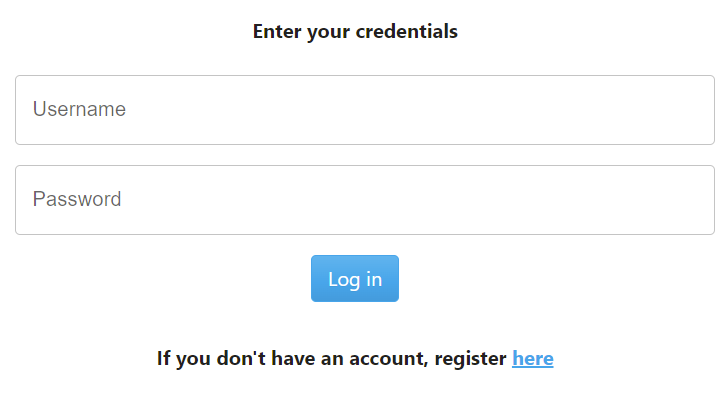
\includegraphics[width=120mm]{images/login-3.png}
	\caption{Login page}
\end{figure}

The user should log in to the system with the correct username and password. Otherwise, error messages will be displayed by explaining what is incorrect with the credentials. If the user does not have an account, he should click on the \emph{here} link which will forward him to the registration page.

\begin{figure}[H]
	\centering
	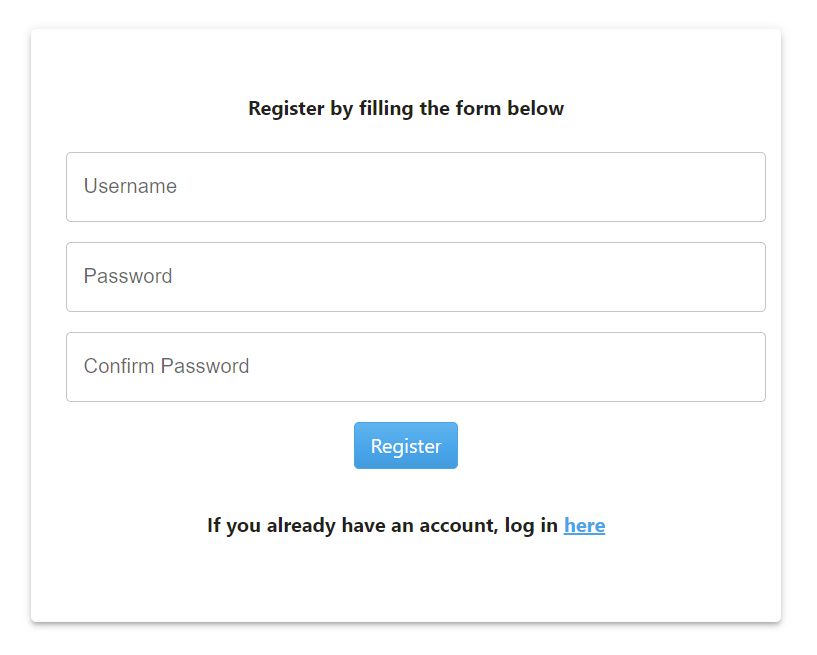
\includegraphics[width=\textwidth]{images/registration.png}
	\caption{Registration page}
\end{figure}

When creating a new account, the user must follow the rules specified below:
\begin{itemize}
  \item \emph{Username} must be unique, size must be between 5 and 15.
  \item \emph{Password} and \emph{Confirm Password} must match, and the size must be between 5 and 15 as well.
\end{itemize}

If the above conditions are not satisfied, error messages will pop up and explain why the user was not been able to create an account. After successful registration, the application will redirect the user to the login page. The user should enter the credentials that were registered previously. Succeeding with logging in will be proceeded by redirecting to \emph{Home Page}.

\begin{figure}[H]
	\centering
	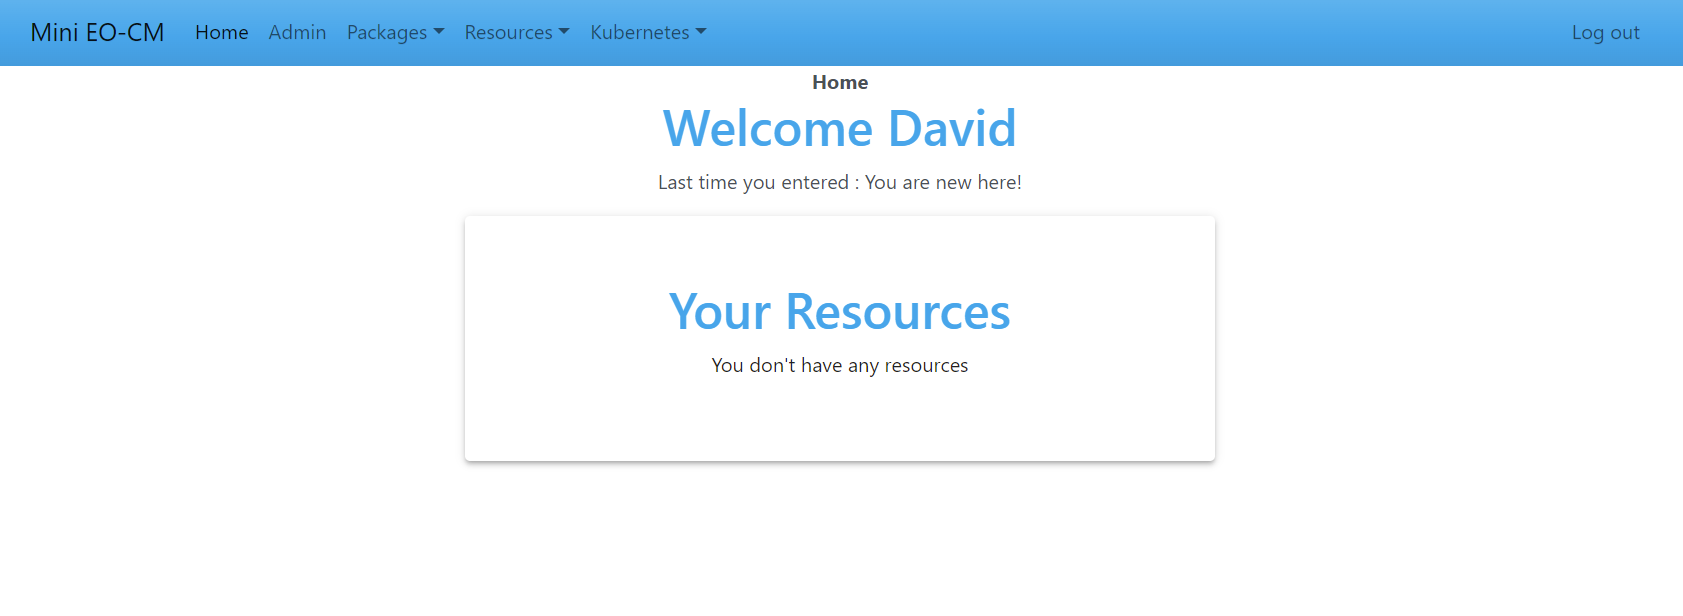
\includegraphics[width=\textwidth]{images/main-1.png}
	\caption{Home page}
	\label{ssec:figure-for-home-page}
\end{figure}

In the header of \emph{Home Page}, there are several menu items arranged. \emph{Home} menu item is the current place of \emph{Home Page}. That is followed by \emph{Admin} page, which is only accessible by Admin users. If the user wants to access \emph{Admin} page, an error message will be displayed.

\begin{figure}[H]
	\centering
	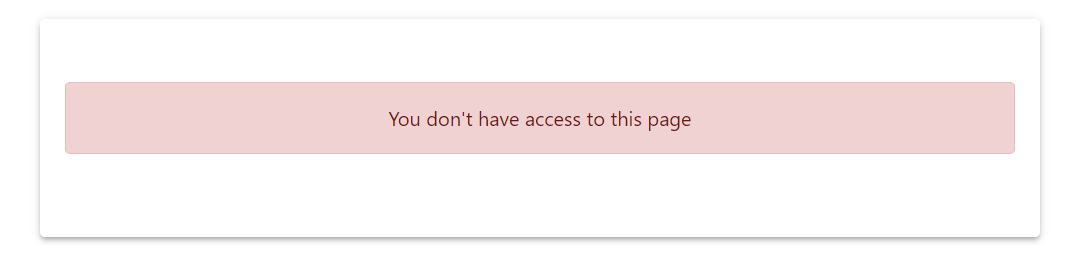
\includegraphics[width=\textwidth]{images/admin-error.png}
	\caption{Not authorized Admin page}
	\label{ssec:admin-authorization}
\end{figure}

If it is the first time user entered the application, \emph{You are new here!} information will be written in \emph{Last time you entered} field. When the user logs out, the application will keep the date and save it in the database. Next time, that date will appear as demonstrated in ~\autoref{ssec:figure-for-home-page-last-date}.

\begin{figure}[H]
	\centering
	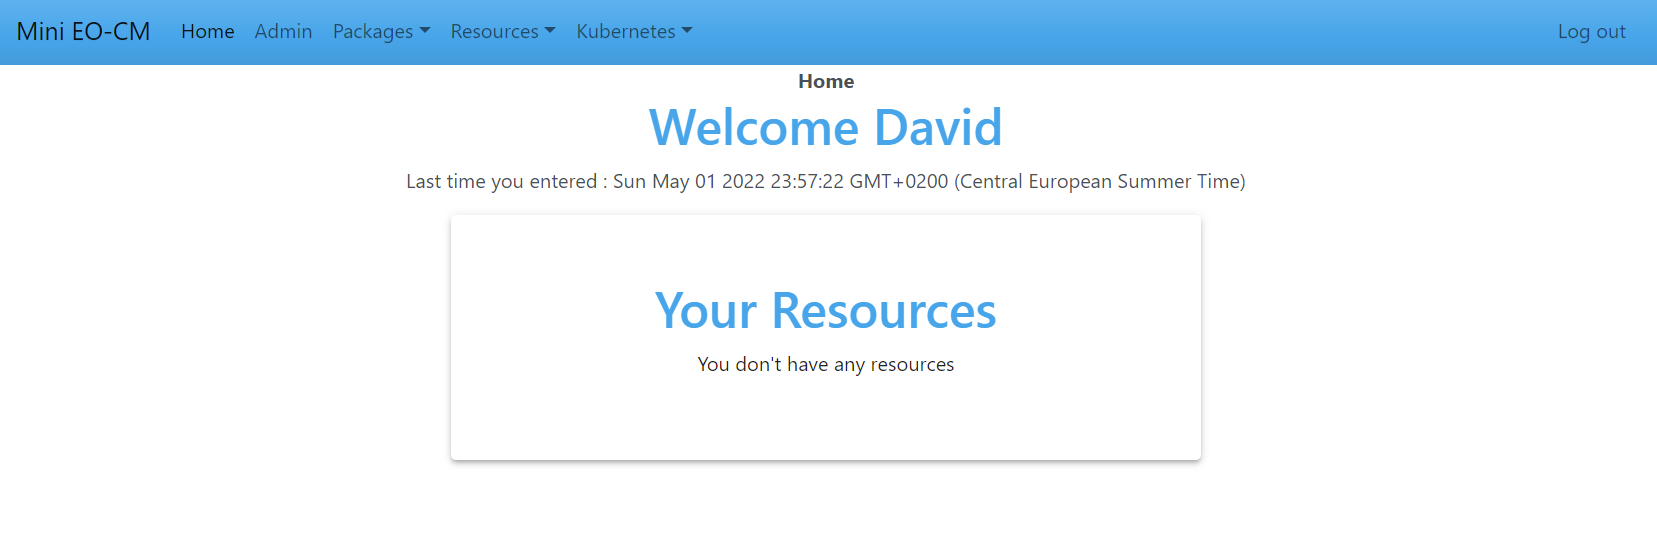
\includegraphics[width=\textwidth]{images/main-2.png}
	\caption{Home page with last entered time}
    \label{ssec:figure-for-home-page-last-date}
\end{figure}

\subsection{Packages}

The next header element is \emph{Packages} menu item, which has 4 operations.

\begin{figure}[H]
	\centering
	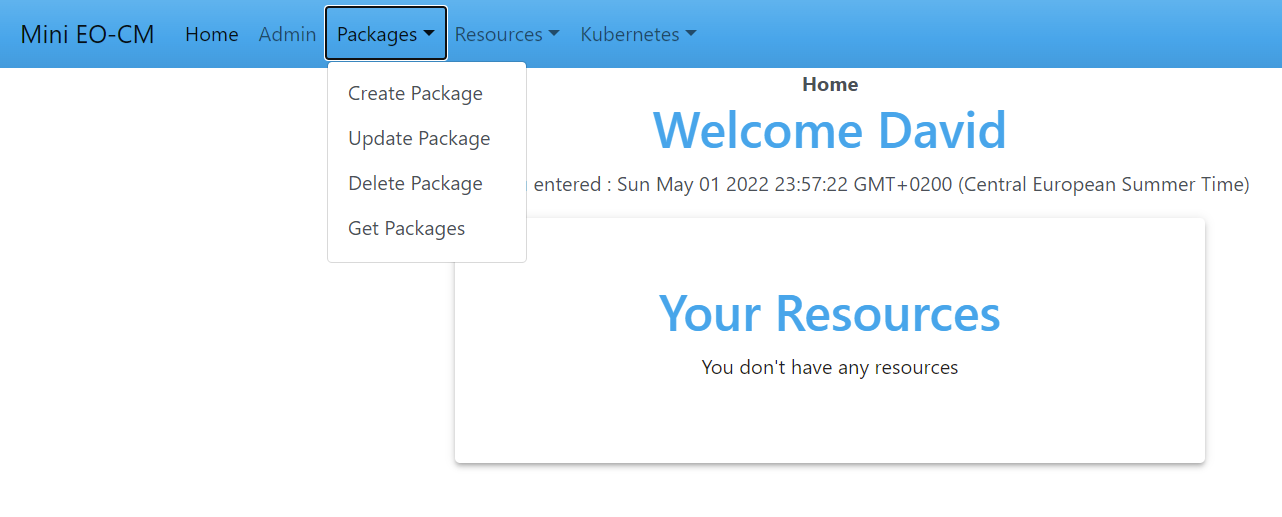
\includegraphics[width=\textwidth]{images/packages-menu.png}
	\caption{Operations on Packages}
	\label{ssec:figure-operations-package}
\end{figure}

\subsubsection{Creating a package}
The user is able to create packages. He should enter the name and type for packages. Application supports 1 type of package for now:
\begin{enumerate}
    \item CNF - used to deploy Container-Based Network Functions into Kubernetes clusters(the Container Infrastructure Service Management (CISM) cluster)
\end{enumerate}

During Package creation rules specified below must be obeyed:
\begin{itemize}
  \item \emph{Package name} size must be between 5 and 15.
  \item \emph{Package type} must be \emph{CNF} package.
\end{itemize}

After the successful creation of the package, the application shows the package ID generated based on the following parameters as illustrated in ~\autoref{ssec:creation-of-package}. By using this ID, the user is able to update and delete this package.

\begin{figure}[H]
	\centering
	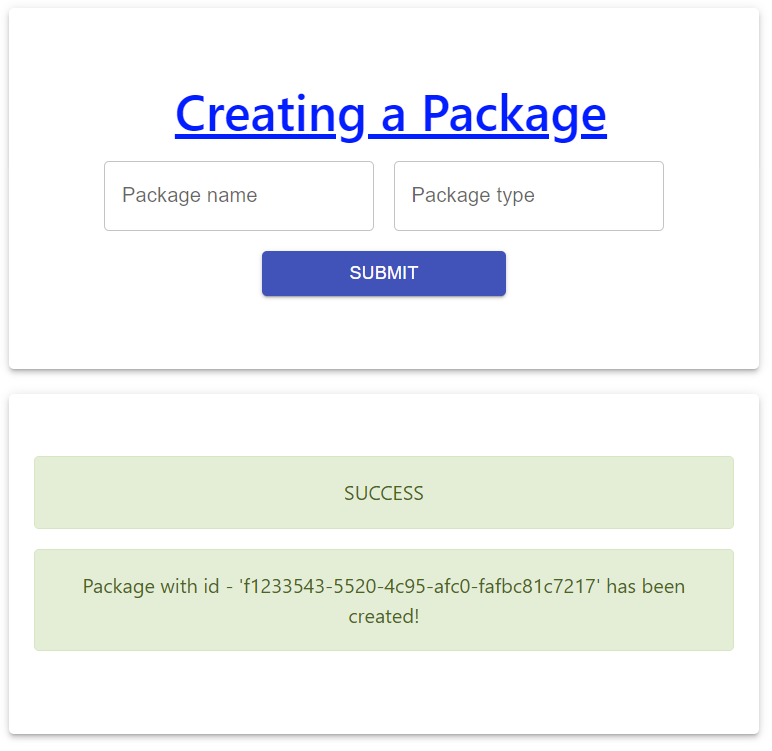
\includegraphics[width=\textwidth]{images/create-package-2.png}
	\caption{Creation of a Package}
	\label{ssec:creation-of-package}
\end{figure}

\subsubsection{List of Packages}
The user is able to see a list of packages created. Here the information about Package ID, name, type as well as creation, and updated time are displayed.

\begin{figure}[H]
	\centering
	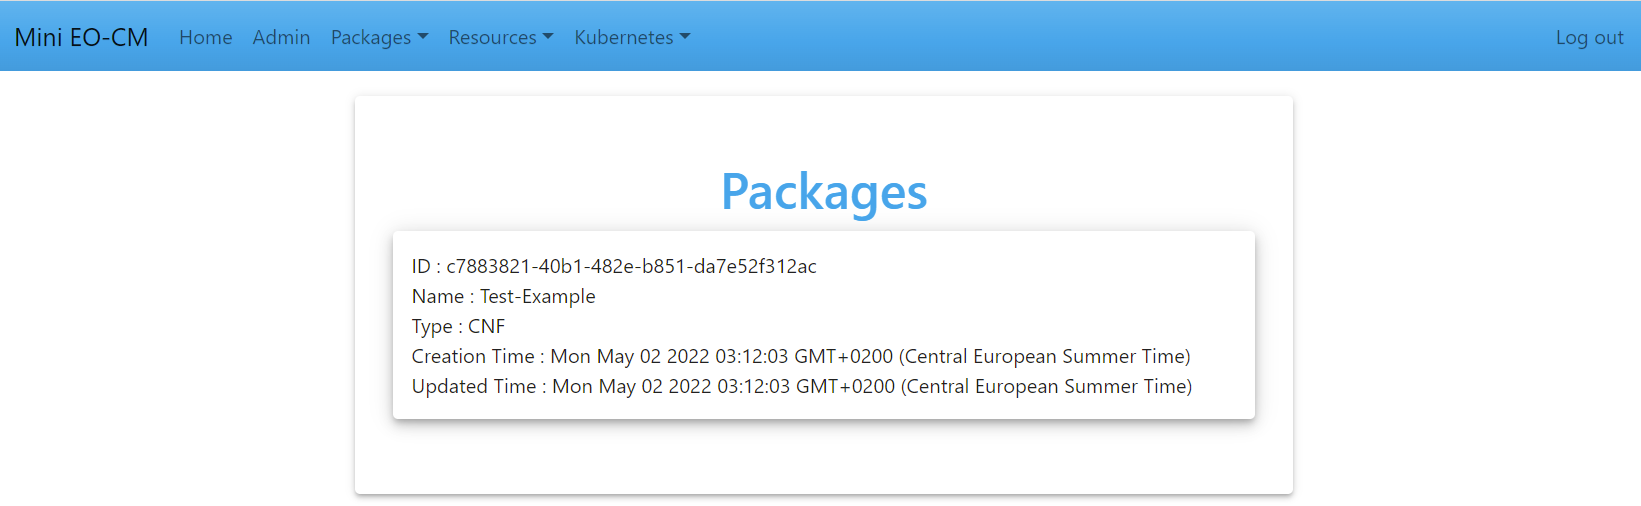
\includegraphics[width=\textwidth]{images/get-packages-4.png}
	\caption{List of Packages}
\end{figure}

\subsubsection{Updating a package}
Packages can be updated if the name or type attributes of the package have been created inaccurately. The rules shown below must be followed:
\begin{itemize}
  \item Package ID must exist.
  \item Package name size must be between 5 and 15.
  \item Package type must be \emph{CNF} package.
  \item There must not be deployed \emph{Resource} that related to this Package.
\end{itemize}

After a successful update of the package, a message will appear describing the package with the following ID that has been updated.
\begin{figure}[H]
	\centering
	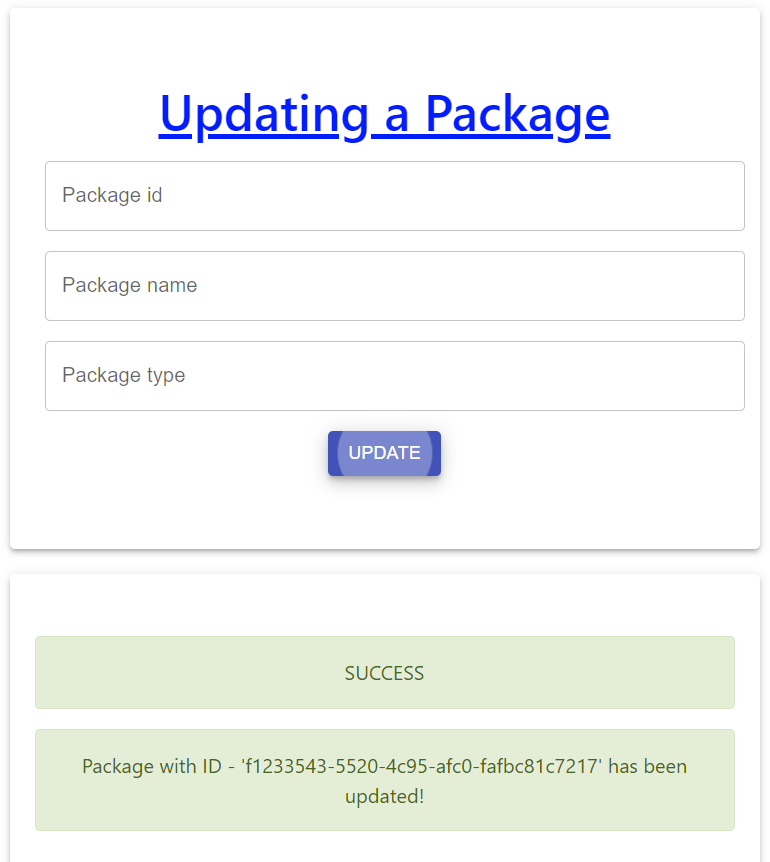
\includegraphics[width=138mm]{images/update-package-2.png}
	\caption{Successful update of a Package}
\end{figure}

\subsubsection{Deleting a package}
Packages can be deleted as well by entering Package ID. The rules shown below must be followed:
\begin{itemize}
  \item Package ID must exist.
  \item There must not be deployed \emph{Resource} that related to this Package.
\end{itemize}

The message, as described in ~\autoref{ssec:deletion-of-package}, will appear by the continuation of successful package deletion. On the condition that the user also had undeployed \emph{Resources} related to this package, they will be deleted as well.

\begin{figure}[H]
	\centering
	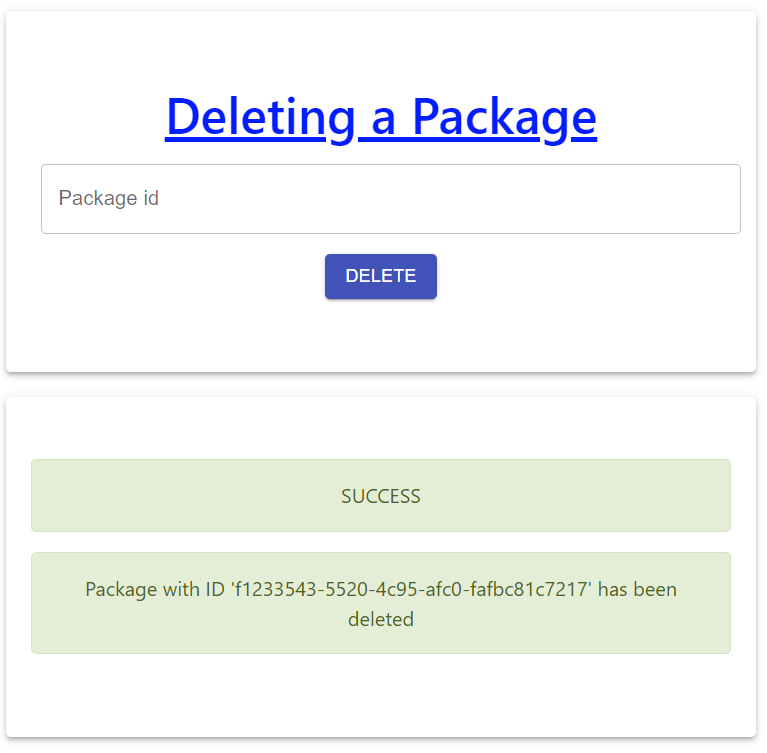
\includegraphics[width=130mm]{images/delete-package-2.png}
	\caption{Deletion of a Package}
	\label{ssec:deletion-of-package}
\end{figure}

\subsection{Resources}
After creating packages and some other operations, based on these packages, Resources can be created which later will be deployed to the Kubernetes. Besides creating a Resource, reading and deleting that resource is also possible.

\begin{figure}[H]
	\centering
	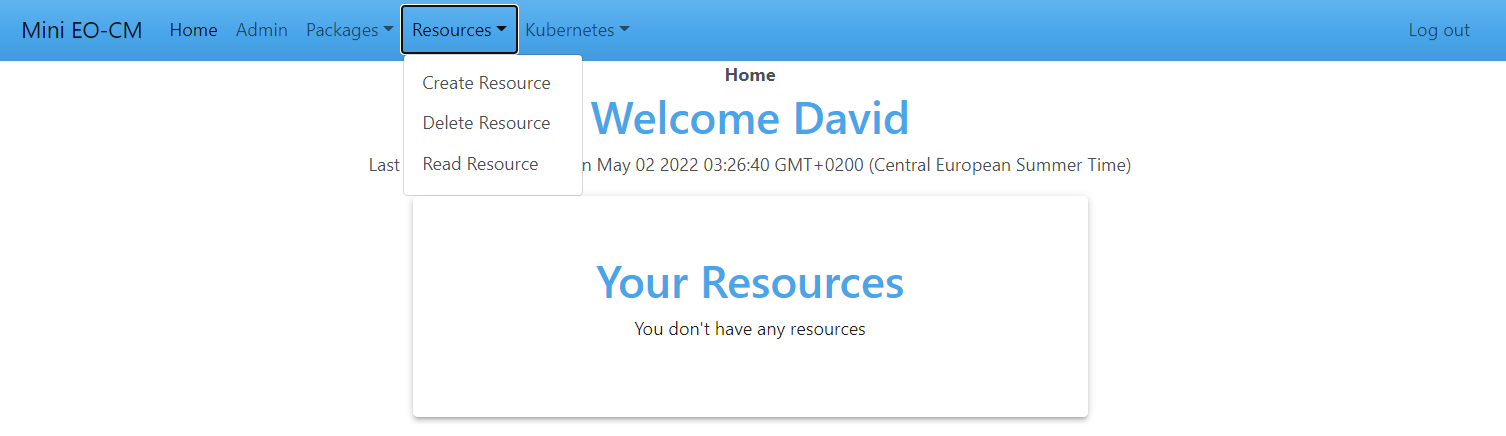
\includegraphics[width=\textwidth]{images/resource-operation.png}
	\caption{Operations on Resource}
	\label{ssec:operations-on-resource}
\end{figure}

\subsubsection{Create a Resource}
Resources can be created based on the Package ID and YAML file. The user generates a YAML file and sends it alongside kind and Package ID. Kind represents the type of Kubernetes objects to be created while using the YAML file. The application supports 6 kinds:
\begin{enumerate}
    \item \textbf{Service} - a REST object in Kubernetes which is similar to a Pod. Like all of the REST objects, a POST HTTP request can be sent for a Service definition to the API server in order to create a new instance. Service object name must be a valid RFC 1035 label name~\cite{rfc-1035}.
    \item \textbf{Deployment} - provides declarative updates for Pods and ReplicaSets. Deployments can be defined to create new ReplicaSets or to detach existing Deployments and adopt all their resources with new Deployments.
    \item \textbf{Job} - can create several Pods. This will be continued until a specified number of retry execution of the Pods successfully terminated. Once pods are complete, the Job tracks the successful completions. The Job is considered complete when a specified number of successful completions is reached
    \item \textbf{ReplicaSet} - The purpose of ReplicaSet is to maintain a steady set of replica Pods running at any given time. In essence, it is frequently used to guarantee the availability of a specified number of identical Pods.
    \item \textbf{StatefulSet} - workload API object used to manage stateful applications.
    Manages the deployment and scaling of a set of Pods, and provides guarantees about the ordering and uniqueness of these Pods.
    \item \textbf{ControllerRevision} - implements an immutable snapshot of state data. Users are responsible for serializing and deserializing the objects that contain their internal state. ControllerRevision can not be updated once it is created.
\end{enumerate}

Example YAML file for each Kubernetes object can be found in \texttt{exampleResources} folder. The rules shown below must be followed when creating a Resource:
\begin{itemize}
  \item Package ID must exist.
  \item Kind must be supported.
  \item If there is already a Resource based on this Package ID, this will replace an already existing resource, nevertheless, the resource must be available.
\end{itemize}

If the above-mentioned conditions are satisfied, then Resource is created and the file is uploaded to the system. On the condition that the kind is not supported or the file is syntactically wrong, then detailed error messages will be displayed.

\begin{figure}[H]
	\centering
	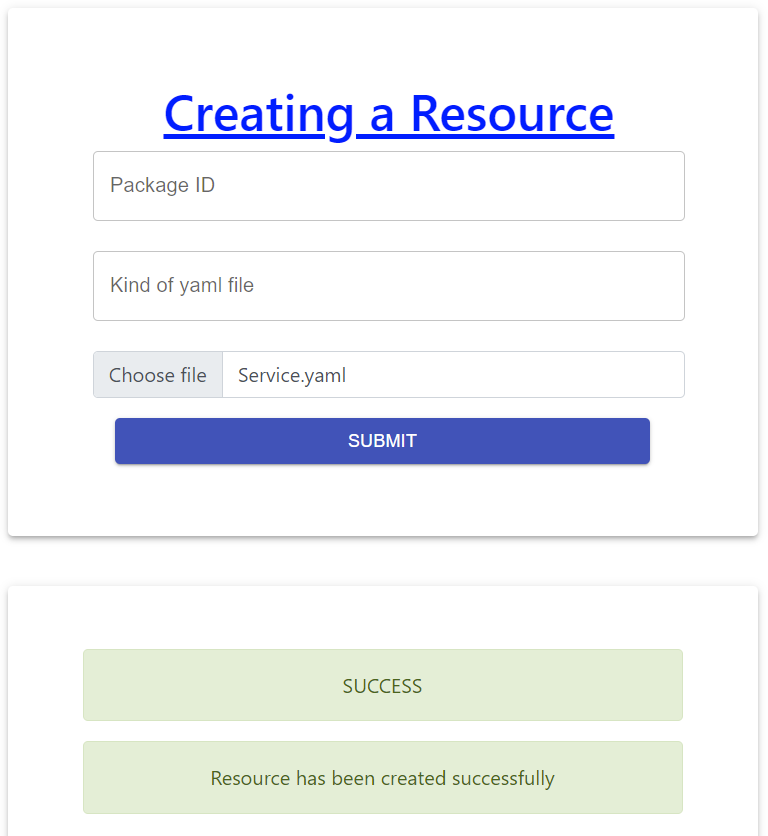
\includegraphics[width=120mm]{images/creation-resource-2.png}
	\caption{Creation of Resource}
	\label{ssec:creation-of-resource}
\end{figure}

After the creation of the Resource, it will be listed on \emph{Home} page, and its relevant Resource ID, Name, Kind, and availability are illustrated for each resource. 

\begin{figure}[H]
	\centering
	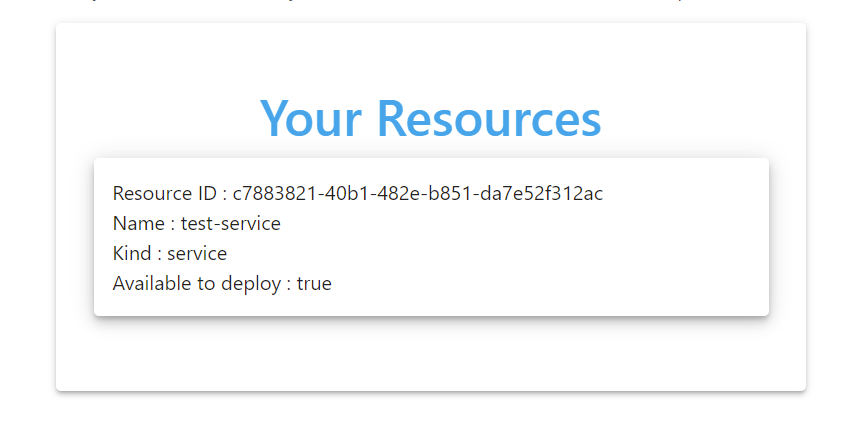
\includegraphics[width=130mm]{images/your-resource-1.png}
	\caption{List of Resources}
	\label{ssec:list-of-resources}
\end{figure}

\subsubsection{Read Resource}
File that has been uploaded to the system by creating a Resource can be viewed by entering relevant Resource ID. 

\begin{figure}[H]
	\centering
	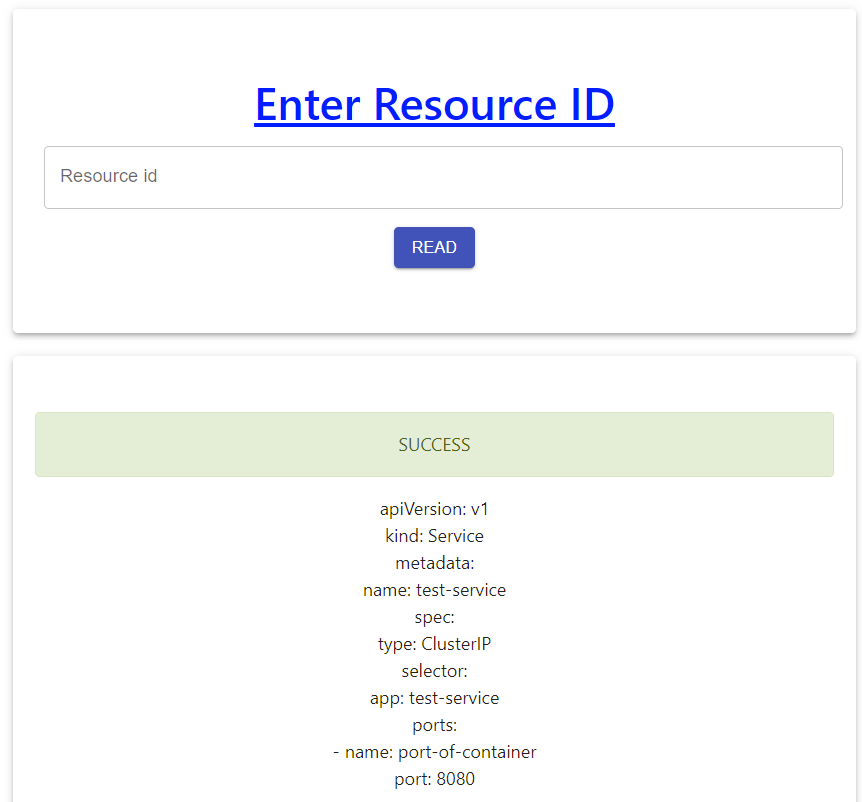
\includegraphics[width=120mm]{images/read-resource.png}
	\caption{Reading a Resource}
	\label{ssec:reading-a-resource}
\end{figure}

\subsubsection{Delete Resource}
A Resource can be deleted by entering the relevant Resource ID. The rules shown below must be followed:
\begin{itemize}
  \item Package ID must exist.
  \item The Resource must be available, it must not be deployed to Kubernetes.
\end{itemize}

The message, as described in ~\autoref{ssec:deleting-a-resource}, will appear by the continuation of successful Resource deletion. The relevant file that has been uploaded will be deleted as well.
\begin{figure}[H]
	\centering
	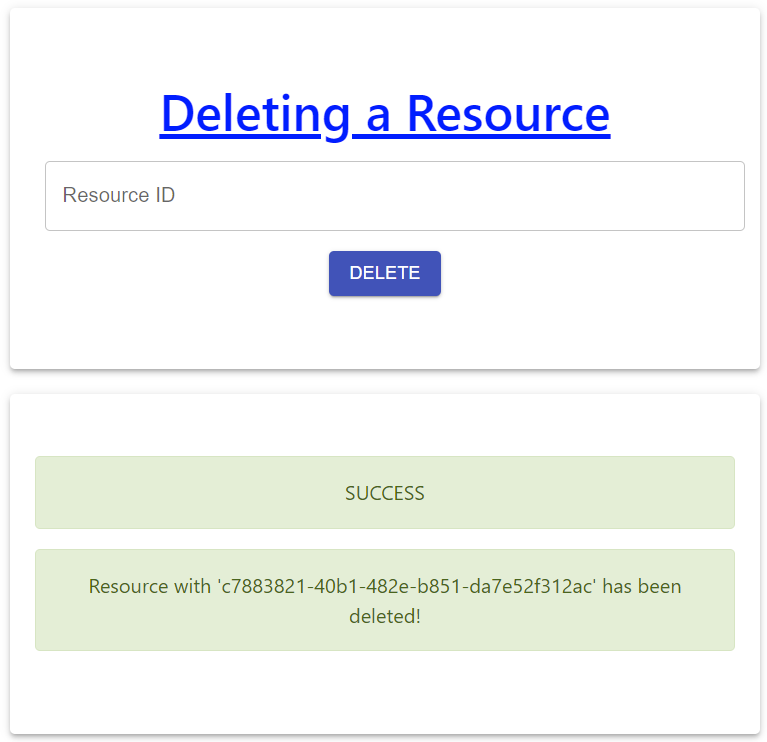
\includegraphics[width=140mm]{images/delete-resource-2.png}
	\caption{Deleting a Resource}
	\label{ssec:deleting-a-resource}
\end{figure}

\subsection{Kubernetes}
\emph{Kubernetes} is the next header element. Users can list all the pods and nodes, can deploy Resources that have been created previously, and delete them. The following subsections explain every operation in a more detailed version.

\begin{figure}[H]
	\centering
	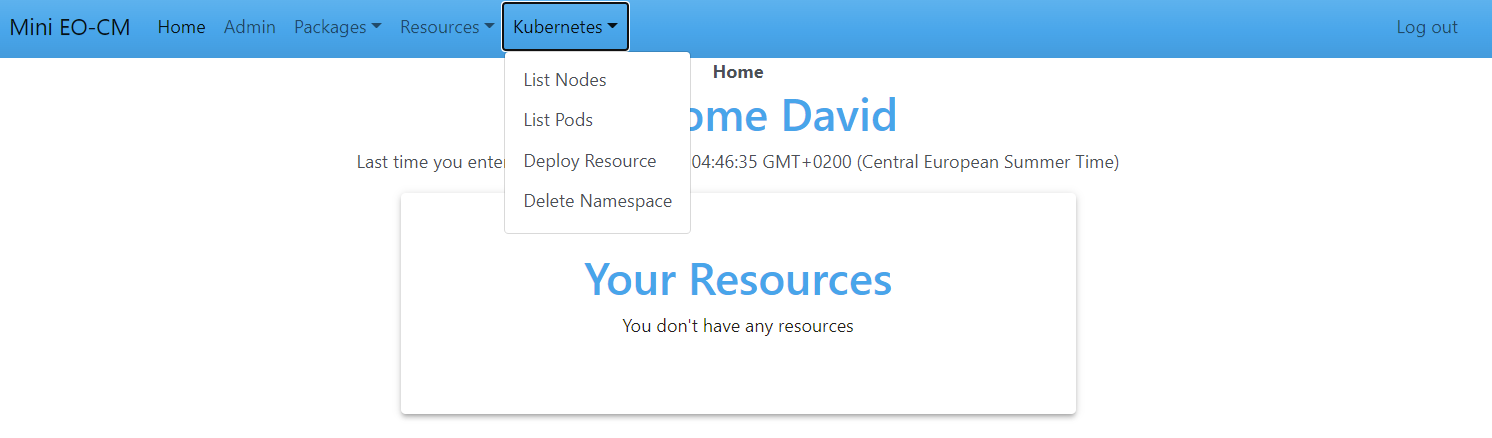
\includegraphics[width=140mm]{images/kubernetes-operations.png}
	\caption{Kubernetes Operations}
	\label{ssec:kubernetes-operations}
\end{figure}

\subsubsection{List Nodes}
Nodes together form a powerful machine. When programs are deployed onto the cluster, the work is distributed to the individual nodes. Name, status, creation time, and version are displayed for each of the nodes.
\begin{figure}[H]
	\centering
	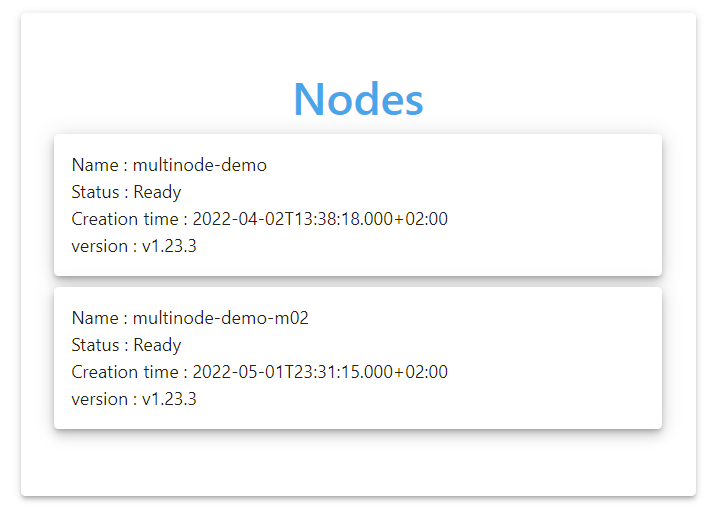
\includegraphics[width=130mm]{images/nodes.png}
	\caption{List of Nodes}
	\label{ssec:list-of-nodes}
\end{figure}

\subsubsection{List Pods}
Kubernetes creates a Pod to host the application instance when a Resource is deployed. Name, status, creation time, and the number of restarts are listed for each of the Pods.
\begin{figure}[H]
	\centering
	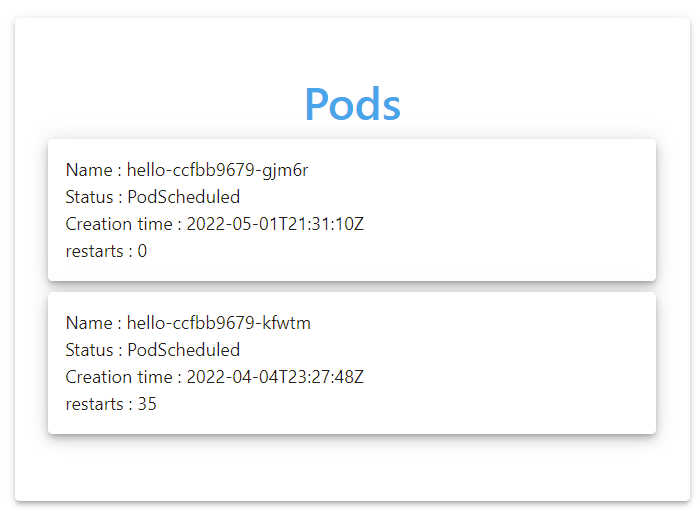
\includegraphics[width=130mm]{images/pods.png}
	\caption{List of Pods}
	\label{ssec:list-of-pods}
\end{figure}

\subsubsection{Deploy Resource}
The user is able to deploy a Resource based on the following rules specified below:
\begin{itemize}
  \item Resource ID must exist.
  \item Resource ID must be available to deploy.
\end{itemize}

\begin{figure}[H]
	\centering
	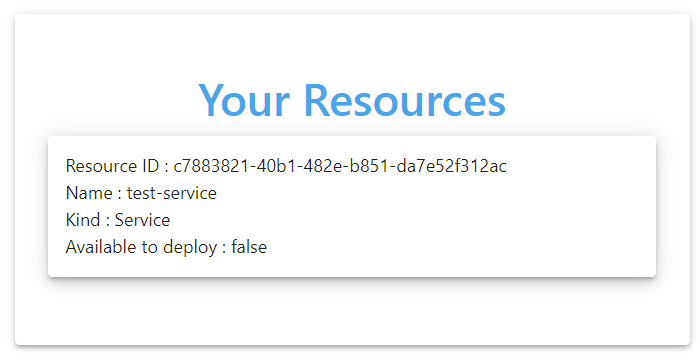
\includegraphics[width=140mm]{images/your-resource-2.png}
	\caption{Resource after deployment}
	\label{ssec:resource-after-deployment}
\end{figure}

If the deployment was successful, the availability of the resource will change from True to False as it is indicated in ~\autoref{ssec:resource-after-deployment}.

\begin{figure}[H]
	\centering
	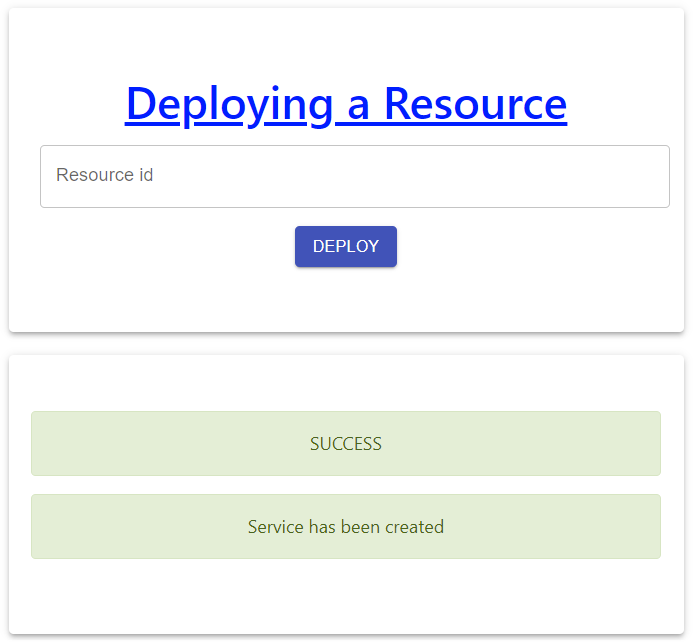
\includegraphics[width=130mm]{images/deploy-service.png}
	\caption{Deploying a Resource}
	\label{ssec:deploy-a-resource}
\end{figure}

\subsubsection{Delete Namespace}
As the user is able to deploy a Resource, deleting that is also possible if the following rules specified below are obeyed:
\begin{itemize}
  \item Resource ID must exist.
  \item Resource ID must be already in deployment state, availability must be False.
\end{itemize}

\begin{figure}[H]
	\centering
	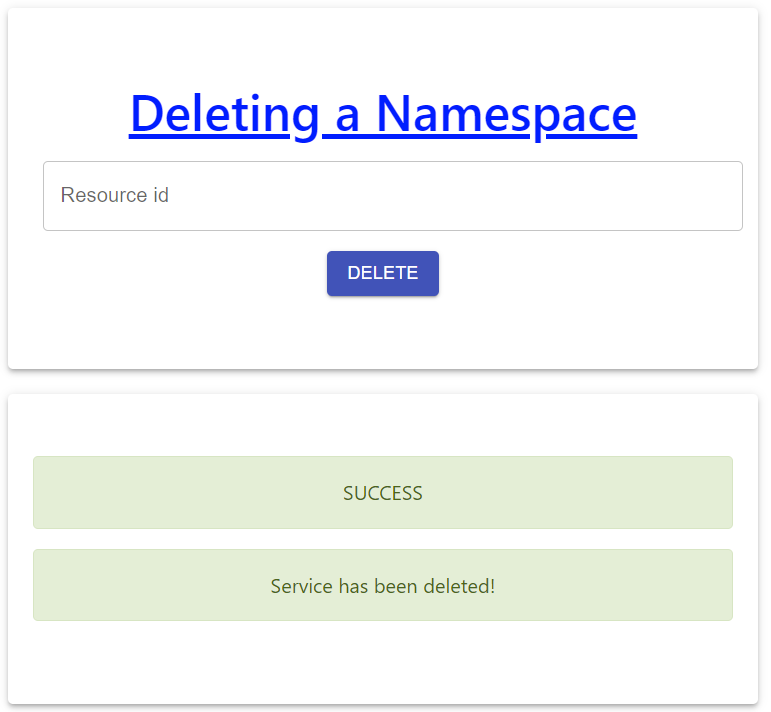
\includegraphics[width=130mm]{images/delete-namespace-2.png}
	\caption{Deleting Namespace}
	\label{ssec:deleting-a-namespace}
\end{figure}

\subsection{Admin}
As discussed earlier in ~\autoref{ssec:admin-authorization}, \emph{Admin} page is designed for administrators to manage the users by listing all information about the users and able to remove them.
Admin can log in to the application with the following credentials:
\begin{itemize}
  \item \emph{Username}: admin
  \item \emph{Password}: admin
\end{itemize}
Username, role and last entered time is displayed for each user in \emph{Admin} page. In order to remove a user, there are some restrictions that exists:
\begin{itemize}
  \item The user must exist
  \item User must not have any \emph{Resources} or \emph{Packages}
  \item Admin cannot remove Admin.
\end{itemize}

If these conditions are fulfilled, the user is deleted successfully, otherwise an error message will be displayed.

\begin{figure}[H]
	\centering
	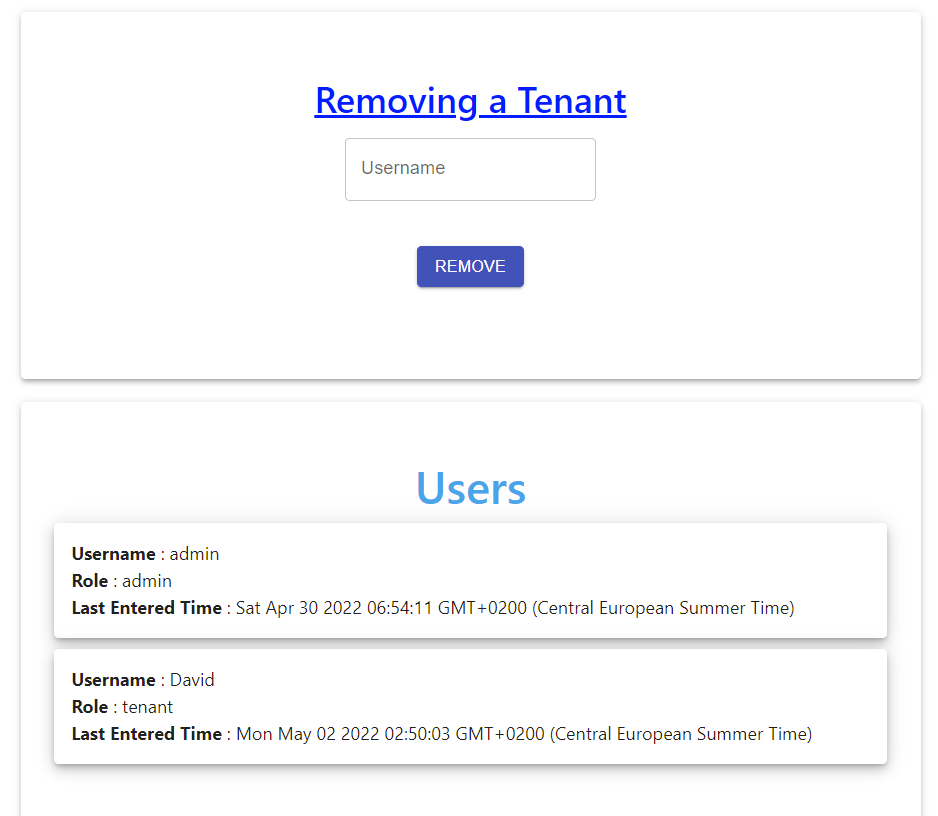
\includegraphics[width=140mm]{images/admin-component.png}
	\caption{Admin page}
	\label{ssec:admin-component}
\end{figure}

This component allows the admin to maintain stability in the application. Most importantly, they ensure a safe and efficient platform where unknown users can be deleted immediately. 

In this chapter, we have introduced the components and usage of the project. Creating packages, uploading YAML files that connect relevant packages, and deploying those resources into Kubernetes is the main accomplishment of the user. Various applications are combined in one GUI and with the help of a few clicks, all the life cycle of network functions virtualization can be done in a second. In the next chapter, we present the models, technology, and implementation of this application.
